\documentclass{beamer}
\beamertemplatenavigationsymbolsempty
\usetheme{Rochester}
\usecolortheme{beaver}
%\usepackage[utf8]{inputenc}
\usepackage[english]{babel}
\parindent=0.pt
\usepackage{amsmath}
\usepackage{graphicx}
\usepackage{verbatim}
\usepackage{tikz}
\usepackage{csquotes}
\usepackage[backend=biber,
style=phys,
citestyle=authoryear
]{biblatex}
\addbibresource{biblio.bib} 
\usepackage[export]{adjustbox}
\usefonttheme[onlymath]{serif}
\newcommand{\R}{\mathbb{R}}
\DeclareMathOperator\supp{supp}
\DeclareMathOperator\shannon{H}
\renewcommand{\qedsymbol}{\includegraphics[width=0.6in, right]{QED Gregory.png}}
\graphicspath{{./Images}/}


\usepackage{tikz}
\newcommand*\circled[1]{\tikz[baseline=(char.base)]{
            \node[shape=circle,draw,inner sep=2pt] (char) {#1};}}


\title{Thermodynamic Costs of Turing Machines \parencite{Kolchinsky_2020}}
\author{Daniel Briseno}

\begin{document}
\frame{\titlepage}

% Introduce the context of the paper and the paper's main purpose

\begin{frame}{Context of the Paper}
\begin{block}{Prior work on Thermodynamics of Information Processing}
\begin{itemize}
    \item Landauer cost of erasing a bit: $kT\ln2$ (1961)
    \item Logically reversible computations can be performed with no heat or entropy production (1973)
    \item Informal argument for minimum cost of $x\mapsto y$ (1989 - 2019)
    \item Development of non-equilibrium statistical physics
    \begin{itemize}
        \item Trajectory-based and stochastic thermodynamics (2013-2015)
    \end{itemize}
    \item Thermodynamic costs of specific implementations of Turing Machines (TM)(2015-2019)
    
    
\end{itemize}
\end{block}
\end{frame}


\begin{frame}{Purpose of the Paper}
    \begin{block}{Thermodynamic costs of computation}
    \begin{itemize}
        \item Extends results to general class of TM
        \item Analyzes the thermodynamic costs of $f:\mathbb{N} \nrightarrow \mathbb{N}$ on a physical implementation of a TM $M$
        \item Logical properties of $f$ and $M$ impose constraints on thermodynamic costs.
        \item Result might generalize to any implementation of a TM
        
    \end{itemize}
    \end{block}
\end{frame}

% Introduce concept of energy from information


\begin{frame}{Heat From Information}
\begin{block}{The Second Law of Thermodynamics}
	\begin{itemize}
	\item Qualitatively, heat cannot flow from a cooler object to a hotter object.
	\item More Quantitatively, there exists a thermodynamic variable $S$, called the entropy, such that:
	\begin{equation*}
	0 \le S_f - S_0 + \Delta Q /T
	\end{equation*}	
	where the RHS of the inequality is called Entropy Production (EP).
	\item An increase in ``order" comes at the cost of producing Heat.
	\end{itemize}
\end{block}
\end{frame}


%Maxwell's demon diagram
\begin{frame}{Heat From Information}
\begin{figure}
	\centering
	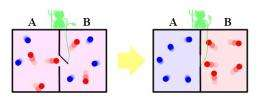
\includegraphics[scale=1]{../Images/maxwellsdemon.jpg}
	\caption{Maxwell's Demon}
	\label{fig:MaxwellsDemon}
\end{figure}
``\textit{... if we conceive of a being whose faculties are so sharpened that he can follow every molecule in its course, such a being, whose attributes are as essentially finite as our own, would be able to do what is impossible to us.}"\\
 \hspace{10mm} -- James Clerk Maxwell
\end{frame}

\begin{frame}{Heat From Information}
\begin{block}{Maxwell's Demon}
\begin{itemize}
	\item Small door can, in principle be opened with 0 EP.
	\item The location of each gas particle can be measured with 0 EP.
	\item Key lies in the demon's memory.
	\begin{itemize}
	\item The Demon must have finite memory.
	\item No matter how well-prepared, eventually the Demon must over-write (erase) one of its memory cells \parencite{bennett_thermodynamics_1982}.
	\end{itemize}
\end{itemize}
\end{block}
\end{frame}

\begin{frame}{Heat From Information}
\begin{block}{Landauer Cost}
\begin{itemize}
	\item The Boltzmann Entropy of a single information-carrying bit is $k\ln(2)$.
	\item The Boltzmann Entropy of a bit that has been erased is 0.
	\item By the second law:
	\begin{align*}
	0 &\le S_f - S_0 + \Delta Q /T\\
	\implies 0 &\le 0 -k\ln(2) + \Delta Q/T\\
	\implies kT\ln(2) & \le \Delta Q
	\end{align*}
	and we obtain the Landauer cost.
\end{itemize}
\end{block}
\end{frame}

%Analysis of Maxwell's Demon


%Introduce concept of Entropy

\begin{frame}{Entropy}
	\begin{block}{Measure of Disorder... Or Energy... Or Information}
		\begin{itemize}
		 	\item Boltzmann Entropy: $S_B = k\ln(w)$
		 	\item Gibbs Entropy: $S_G = -k\sum_i P_i \ln(P_i)$
		 	\item Shannon Entropy: $\shannon = -\sum_i P_i \ln(P_i)$
		\end{itemize}
	\end{block}
\end{frame}

\begin{frame}{Entropy}
\begin{figure}
	\centering
	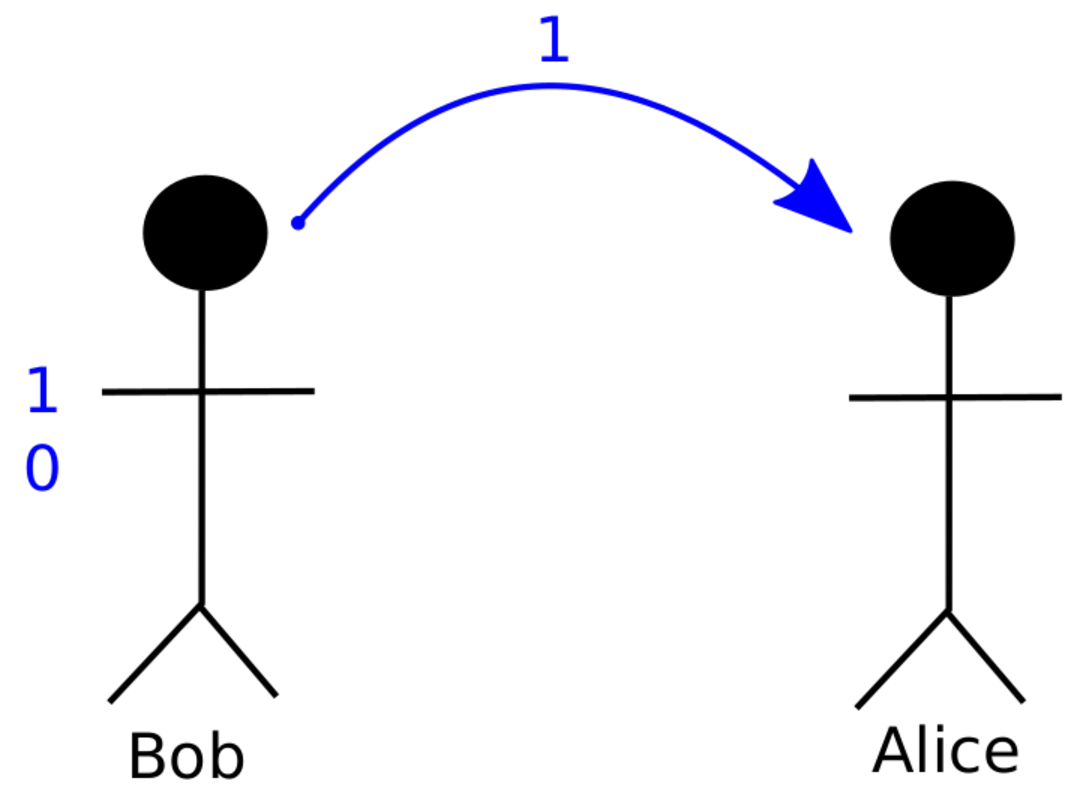
\includegraphics[height=2.5cm]{alice_and_bob.pdf}
	\caption{A tale as old as time.}
	\label{fig:alice_and_bob}
\end{figure}
\begin{block}{Information Content}
\begin{itemize}
	\item How much information does Bob's message give Alice?
	\item More quantitatively, given $\Gamma := \{0,1\}$
	\begin{equation*}
		I: \Gamma \to \R
	\end{equation*}
\end{itemize}
\end{block}
\end{frame}

\begin{frame}{Entropy}
\begin{block}{Case 1}
\begin{figure}
	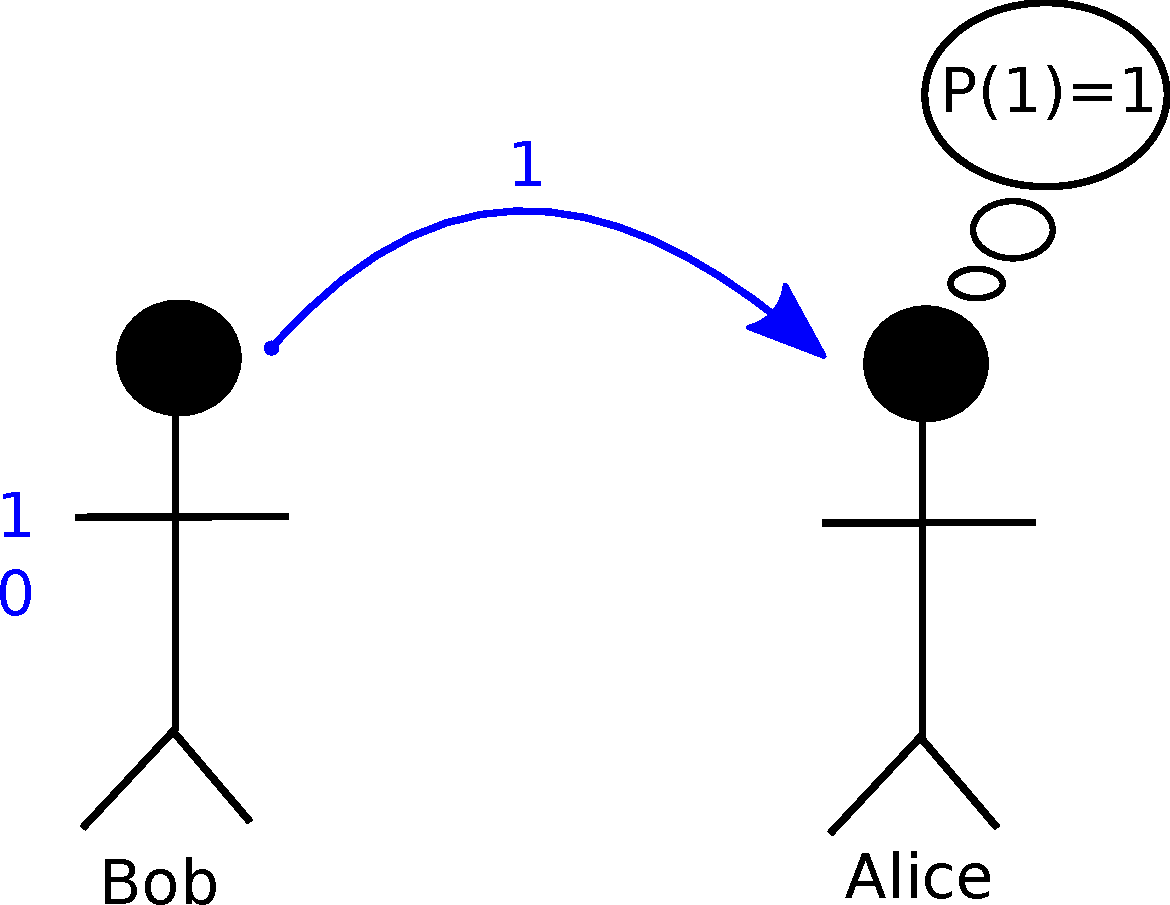
\includegraphics[height=3cm] {alice_and_bob_s1.pdf}
	\label{fig:alice_and_bob_s1}
\end{figure}
\end{block}
\end{frame}

\begin{frame}{Entropy}
\begin{block}{Case 1 cont.}
\begin{figure}
	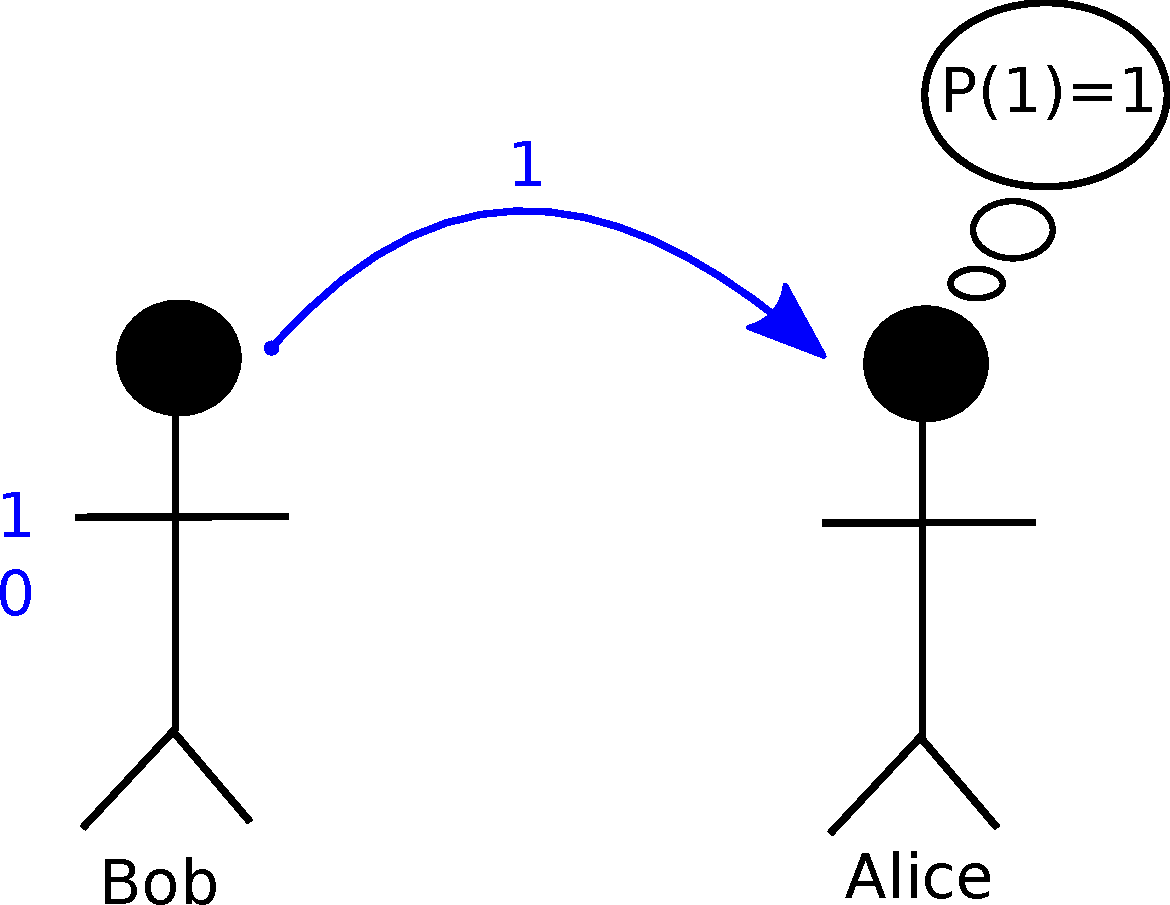
\includegraphics[height=3cm] {alice_and_bob_s1.pdf}
	\label{fig:alice_and_bob_s1_1}
\end{figure}
\begin{itemize}
	\item Bob's message provides no information.
	\item $I(1) = 0$
\end{itemize}
\end{block}
\end{frame}

\begin{frame}{Entropy}
\begin{block}{Case 2}
\begin{figure}
	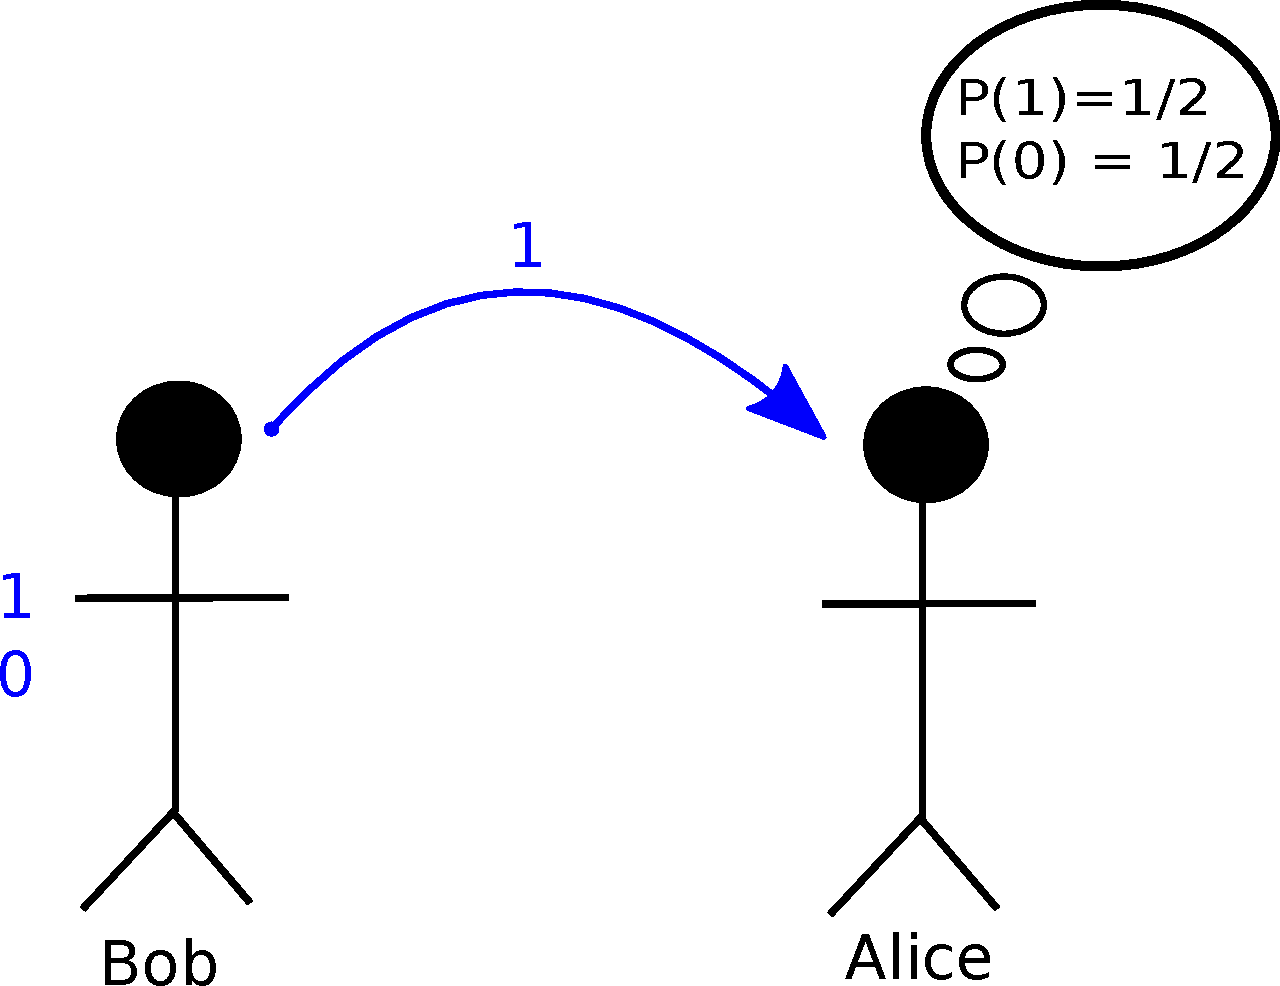
\includegraphics[height=3cm] {alice_and_bob_s2.pdf}
	\label{fig:alice_and_bob_s2}
\end{figure}
\end{block}
\end{frame}


\begin{frame}{Entropy}
\begin{block}{Case 2 cont.}
\begin{figure}
	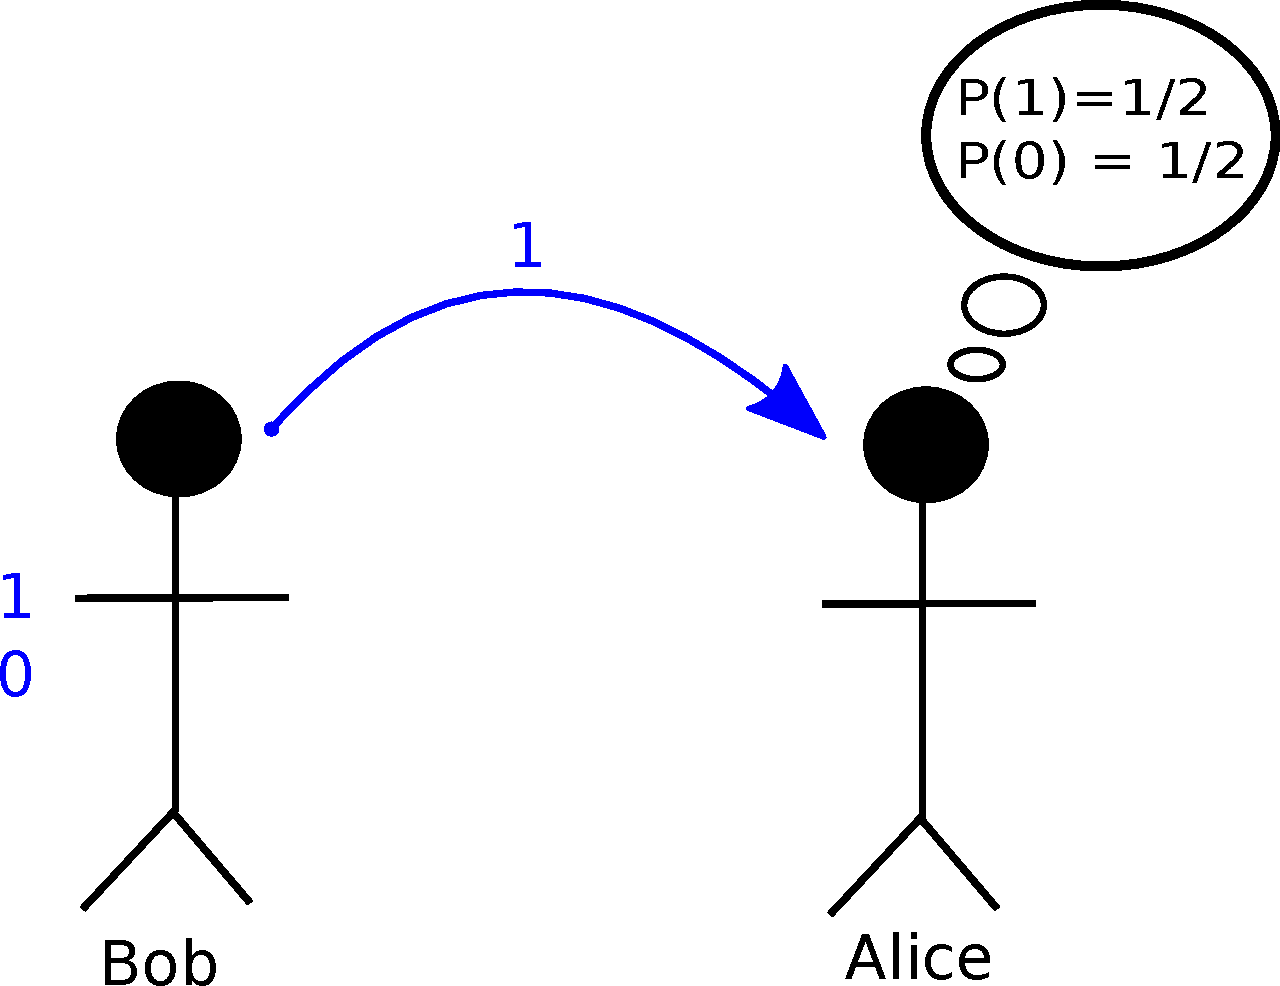
\includegraphics[height=3cm] {alice_and_bob_s2.pdf}
	\label{fig:alice_and_bob_s2_1}
\end{figure}
\begin{itemize}
	\item Bob's message provides one bit of information
	\item $0<I(1)= 1$bit
\end{itemize}
\end{block}
\end{frame}

\begin{frame}{Entropy}
\begin{block}{Case3}
\begin{figure}
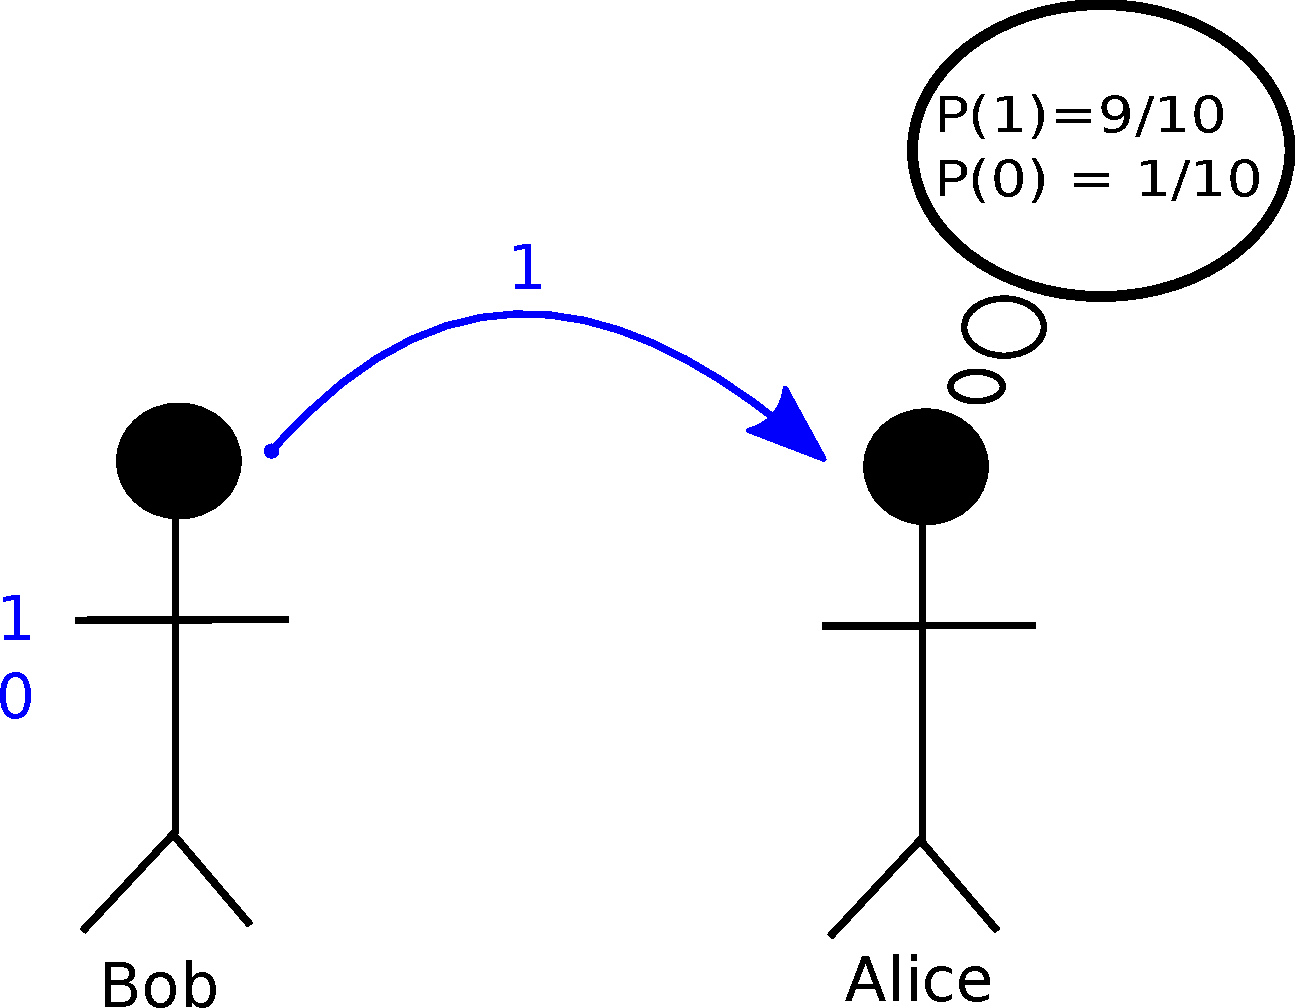
\includegraphics[height=3cm]{alice_and_bob_s3.pdf}
\label{fig:alice_and_bob_s3}
\end{figure}
\end{block}
\end{frame}

\begin{frame}{Entropy}
\begin{block}{Case 3}
\begin{figure}
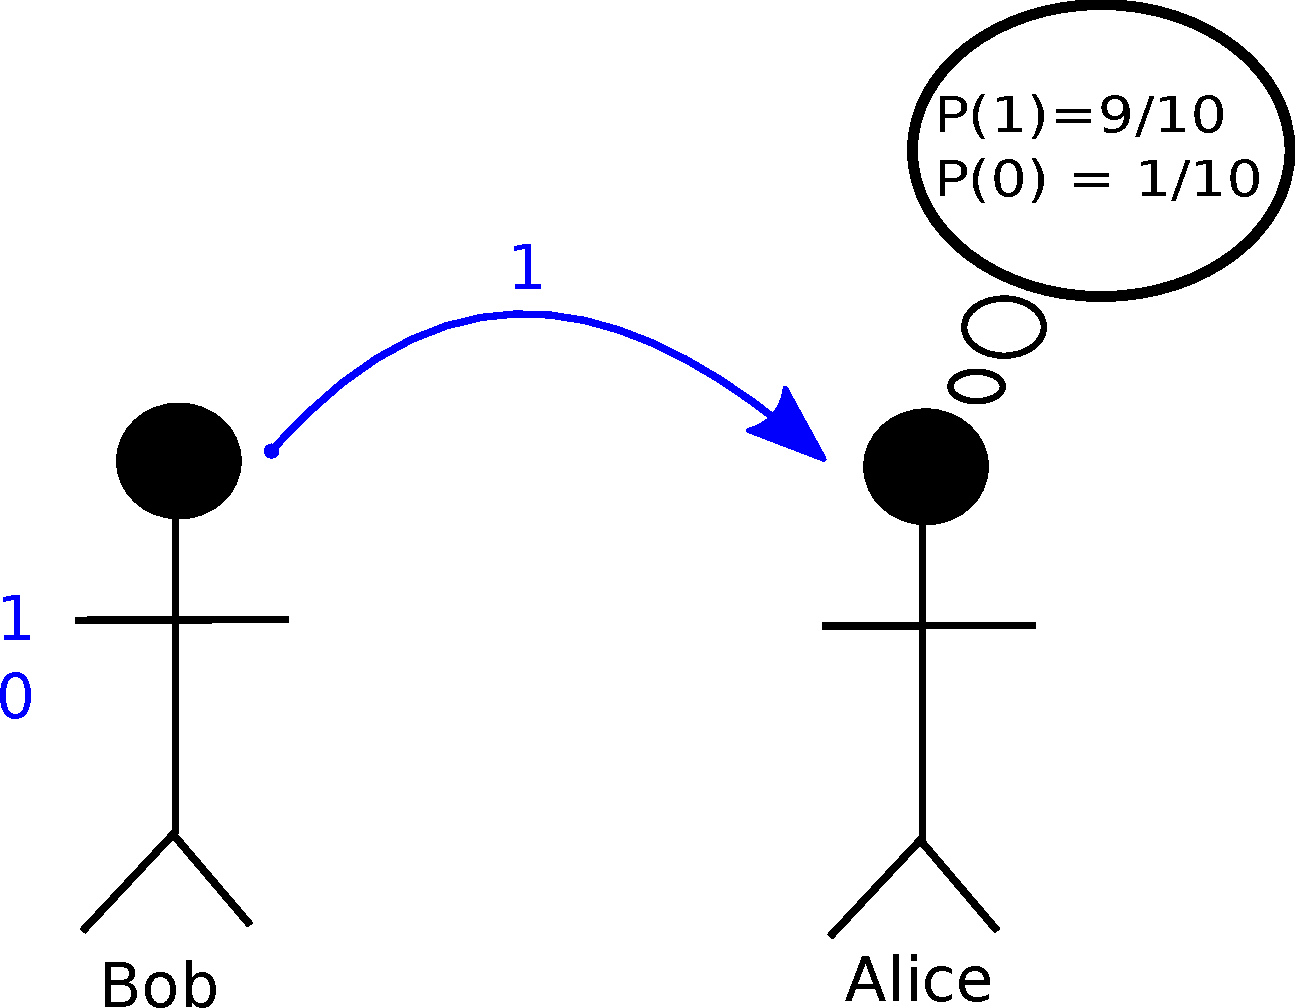
\includegraphics[height=3cm]{alice_and_bob_s3.pdf}
\label{fig:alice_and_bob_s3_1}
\end{figure}
\begin{itemize}
	\item Bob's message removes some uncertainty
	\item Not as informative as in case 2
	\item $0=I^{(1)}(1) < I^{(3)}(1) < I^{(2)}(1)= 1$bit
\end{itemize}
\end{block}
\end{frame}

\begin{frame}{Entropy}
\begin{block}{Case 4}
\begin{figure}
\centering
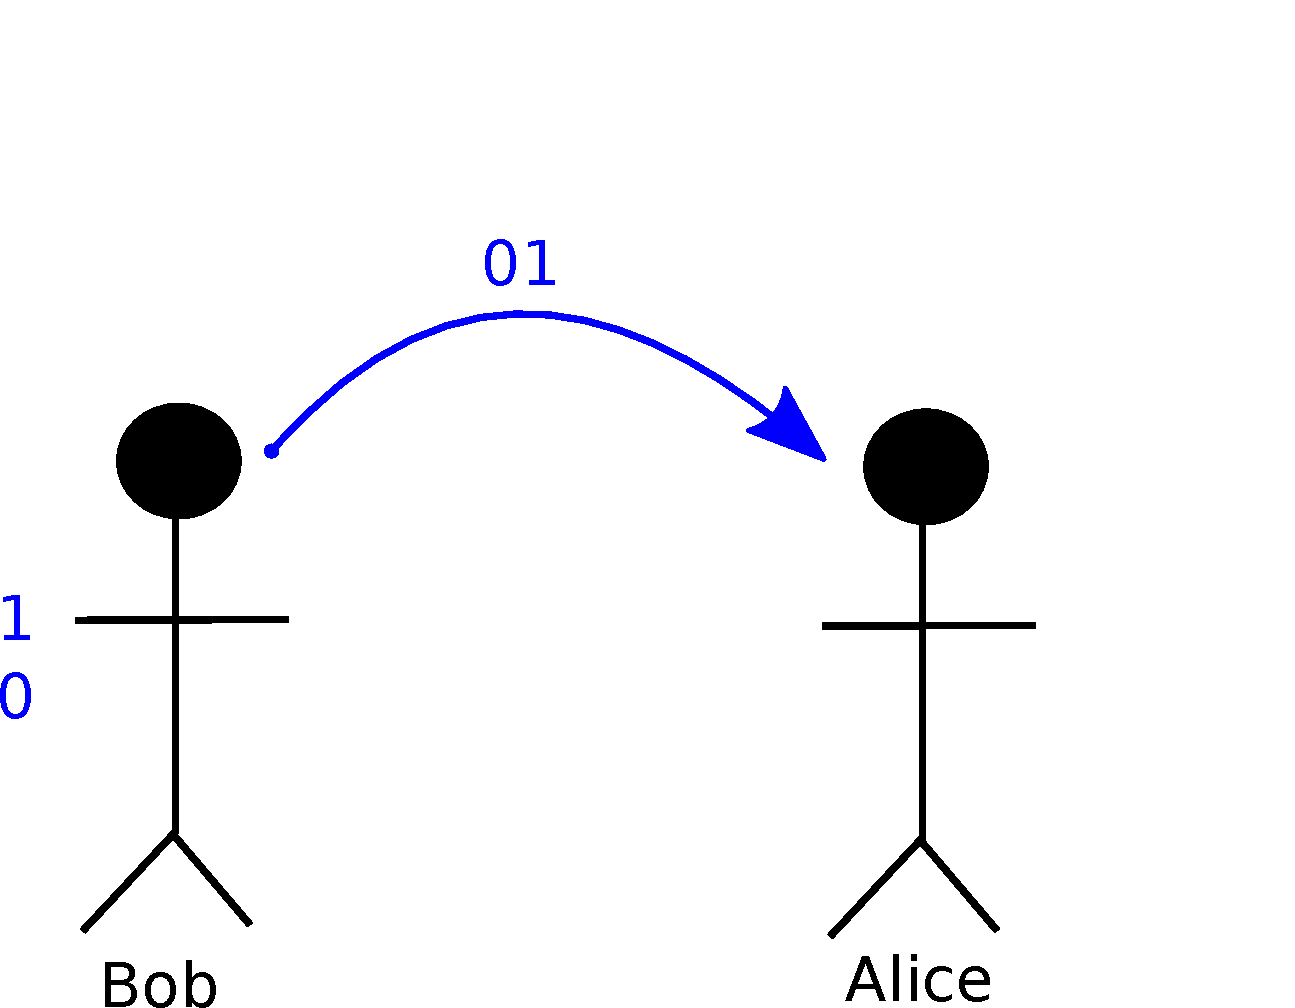
\includegraphics[height=4cm]{alice_and_bob_s4.pdf}
\label{fig:alice_and_bob_s4}
\end{figure}
\begin{itemize}
	\item Decision to send 0 independent from decision to send 1
	\item $I(0,1) = I(0) + I(1)$
\end{itemize}
\end{block}
\end{frame}

\begin{frame}{Entropy}

\begin{block}{ Three Conditions}
For any $x,y \in \Gamma$, the following three axioms must hold:
\begin{enumerate}
	\item $P(x) = 1 \; \implies \; I(x)=0$
	\item $P(x) < P(y) \; \implies \; I(y) < I(x)$
	\item $I(xy) = I(x) + I(y)$
\end{enumerate}
\end{block}
\end{frame}

\begin{frame}{Entropy}
\begin{block}{Information Content, or Surprisal}
Single function which can satisfy these three axioms \parencite{shannon_mathematical_nodate}
\begin{equation*}
I(x) = -\log_b(P_x)
\end{equation*}
Where we write $P_x=P(x)$ for notational simplicity.
\begin{itemize}
	\item This value is called the \textbf{Surprisal}, or \textbf{Information Content}
	\item $b$ sets our units of information
\end{itemize}
\end{block}
\end{frame}

\begin{frame}{Entropy}
\begin{block}{The Bit: $b=2$}
\begin{itemize}
\item If $P(1)=P(2) = 1/2$, then $I(1)=1$ bit.
\begin{align*}
	I_2(1) &= -\log_2(P_1)\\
	&= - \log_2\left(\frac{1}{2}\right)\\
	&= 1
\end{align*}
\end{itemize}
\end{block}
\end{frame}

\begin{frame}{Entropy}
\begin{block}{The nat: $b=e$}
\begin{itemize}
	\item Recall the Boltzmann Entropy $S_B$:
	\begin{equation*}
		S_B = k\ln (w)
	\end{equation*}
	\item $P(w_0) = 1/w$. Thus
	\begin{align*}
		S_B &= -k\ln(P_{w_0})\\
		&= kI_e(w_0)
	\end{align*}
\end{itemize}
\end{block}
\end{frame}

\begin{frame}{Entropy}
\begin{block}{Unit Conversions}
	All $I_b$ are related by the logarithm change-of-base formula:
	\begin{equation*}
	I_c = \frac{1}{\log_b c} I_b
	\end{equation*}
	the factor $\frac{1}{\log_b c}$ can be thought of as a conversion factor.
\end{block}
\end{frame}




\begin{frame}{Entropy}
\begin{figure}
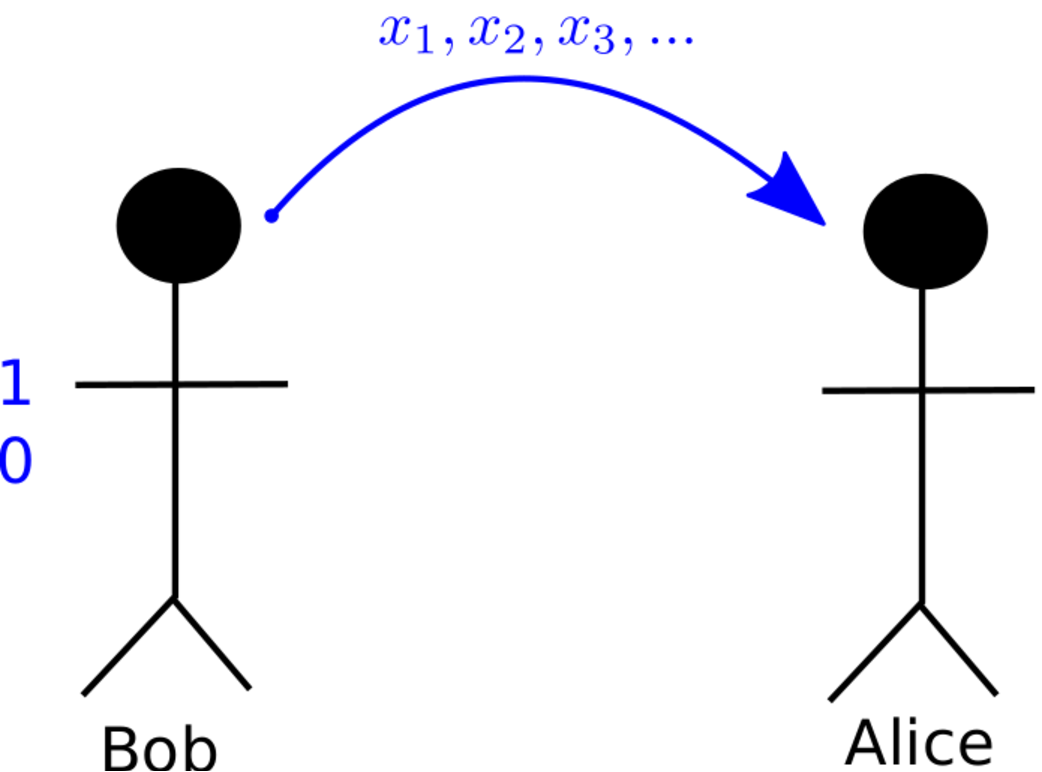
\includegraphics[height=2.5cm]{alice_and_bob_channel.pdf}
\end{figure}
\begin{block}{Shannon Entropy}
\begin{itemize}
	\item Single message replaced with message random variable $X$
	\item How informative is Bob to Alice?
	\item Expected value of Suprisal:
	{\small
	\begin{align*}
		\shannon(X) &= - \sum_{i=1}^2 P_{i} \log_2(P_{i})\\
		&= \mathbb{E}[I_2(X)]
	\end{align*}}
\end{itemize}
\end{block}
\end{frame}



\begin{frame}{Entropy}
\begin{block}{Gibbs Entropy}
\begin{figure}
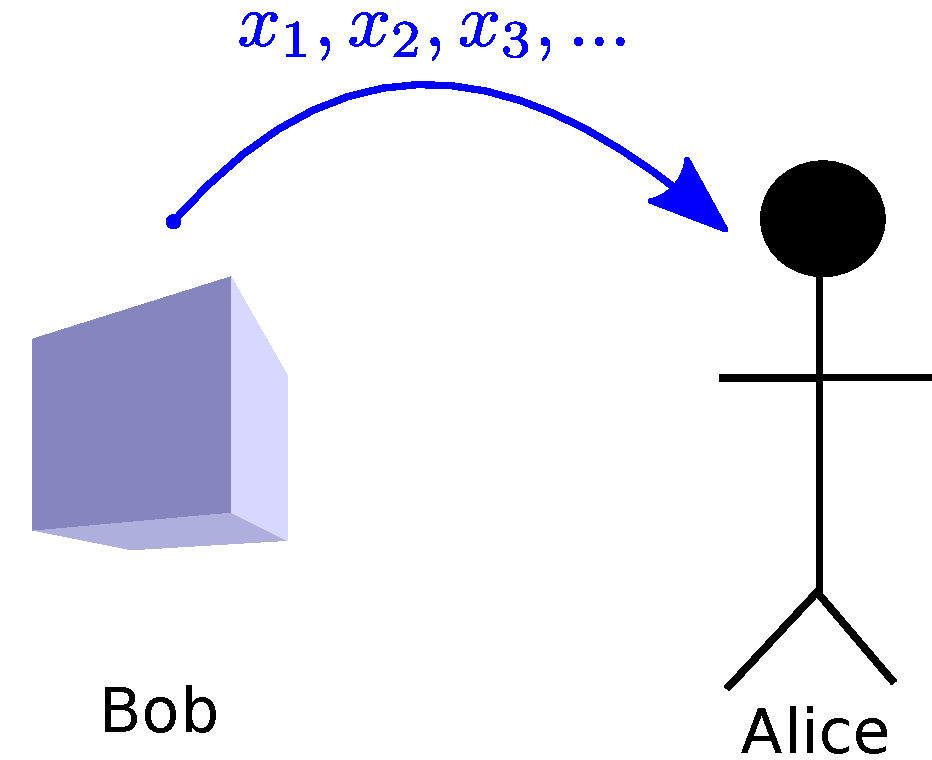
\includegraphics[height=3cm]{alice_and_bob_system.pdf}
\end{figure}
\begin{itemize}
	\item We replace the message alphabet $\Gamma$ with a finite state-space $\chi$
	\begin{align*}
		S_G &= -k \sum_{x\in\chi}P_x \ln(P_x)\\
		&= k \mathbb{E}[I_e(X)]
	\end{align*}
\end{itemize}
\end{block}
\end{frame}

\begin{frame}{Entropy}
\begin{block}{Types of Entropies Revisited}
For a system with state-space $\chi$, $x\in\chi$, and random variable $X$ with support $\chi$:
\begin{itemize}
	\item Information Content: $I_b(x) = - \log_b(P_x)$
	\item Boltzmann Entropy: $S_B = kI_e(w_0)$
	\item Shannon Entropy: $\shannon = \mathbb{E}[I_b(X)]$
	\item Gibbs Entropy: $S_B = k\mathbb{E}[I_e(X)] = k\shannon_e$ 
\end{itemize}
\end{block}
\end{frame}


\begin{frame}{Entropy}
\begin{block}{Maxwell's Demon Revisited}
\begin{itemize}
	\item Boltzmann entropy of a information-carrying bit:
	{\small
	\begin{align*}
		w_0 &= 1\\
		kI_e(1) &= -k\ln(P_1) = k\ln(2)
	\end{align*}}
	\item Boltzmann entropy of a bit overwritten with 0:
	{\small
	\begin{align*}
		w_0 &= 0\\
		kI_e(0) &= 0
	\end{align*}}
	\item Second law implies:
	{\small
	\begin{align*}
		0 &\le 0 - k\ln(2) + \Delta Q/T\\
		\implies kT\ln(2) &\le \Delta Q
	\end{align*}
	}
\end{itemize}
\end{block}
\end{frame}




















% Introduce Turing Machines and other CS background
\begin{frame}{CS Background}
    \begin{block}{Turing Machines}
        \begin{figure}
            \centering
            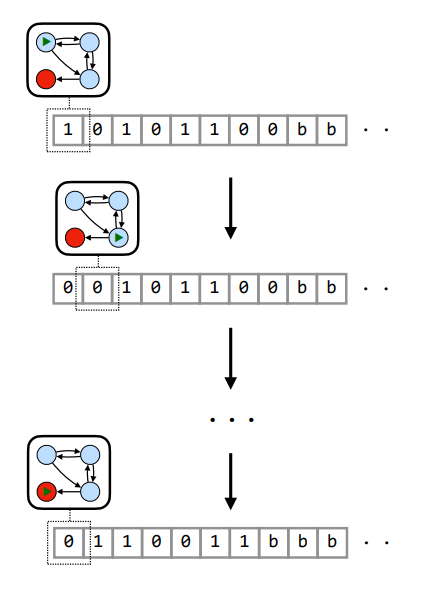
\includegraphics[height=5cm]{TM.png}
            \caption{Graphical representation of a TM}
            \label{fig:my_label}
        \end{figure}
    \end{block}
\end{frame}

\begin{frame}{CS Background}
\begin{block}{Turing Machines}
Formal definition of a Turing Machine:
    \begin{itemize}
        \item A Turing machine $M$ is a 4-tuple $M = (Q,\Sigma, q_0,\delta) $ where:
        \begin{itemize}
            \item $Q$ is a finite nonempty set of states.
            \item $\Sigma$ is a finite nonempty set of symbols.
            \item $q_0\in Q$ is the initial state of $M$
            \item $\delta: (Q\times \Sigma) \nrightarrow (\Sigma \times \{L,R\}\times Q)$ is a partial transition function determining the symbol written on the tape, the movement of the read-write head, and the next state of the $M$.
        \end{itemize}
    \end{itemize}
\end{block}
\end{frame}

\begin{frame}{CS Background}
    \begin{block}{Additional Assumptions on TM $M$}
    
    \begin{enumerate}
        \item $\Sigma = \{0,1,b\}$
        \item If and when $M$ halts on an input, the tape will contain an output string $s\in \{0,1\}^*$ followed by all blank symbols, and the pointer will be set to the start of the tape.
    \end{enumerate}
    Assumptions do not affect the computational capabilities of $M$.
    \end{block}
\end{frame}
    
\begin{frame}{CS Background}
    \begin{block}{Turing Machines as Partial Functions}
    Any computation performed by a TM $M$ can be represented as
    \begin{equation*}
        \phi_M:\{0,1\}^* \nrightarrow \{0,1\}^*
    \end{equation*}
    and $\phi_M(x) = y$ indicates that $M$ started with input program $x$ yields the output string $y$.
    \end{block}
    \begin{block}{Universal TM}
    There exist Universal Turing Machines (UTM) such that given a UTM $U$ and any TM $M$, there exists an interpreter program $\sigma_{U,M}$ such that
    \begin{equation*}
        \phi_U(\sigma_{U,M},x) = \phi_M(x)
    \end{equation*}
    \end{block}
\end{frame}

\begin{frame}{CS Background}
\begin{block}{The Print function, an example}
\begin{itemize}
	\item There exists a FPGA (Field-programmable-gate-array) which constitutes a circuit capable of parroting back any binary string fed to it.
	\item This computer is also capable of printing out a binary string.
\end{itemize}
\end{block}
\end{frame}

\begin{frame}{CS Background}
\begin{block}{The Print function, an example}
	\begin{itemize}
		\item $\phi_D$ UTM which models my personal computer
		\item $\phi_M$ TM which models a "print" FPGA
		\item $x$ binary string which $\phi_M$ can print
		\item $\sigma_{D,M}$ interpreter program
		\item $(\sigma_{D,M},x)$ input to my UTM $\phi_D$
	\end{itemize}
\end{block}
\end{frame}

\begin{frame}{CS Background}
\begin{block} {TM input}
\begin{itemize}
	\item The input to a TM is not generally the input to a program
	\item The input to a TM is the program itself, along with any necessary parameters
\end{itemize}
\end{block}
\end{frame}

\begin{frame}{CS Background}
    \begin{block}{Computability}
    \begin{itemize}
        \item Church Turing Thesis: A function can be calculated by a sequence of formal operations if and only if it is computable by a Turing Machine.
       \item Physical Church Turing Thesis: Any function implemented by a physical process can also be implemented by a Turing Machine
    \end{itemize}
    \end{block}
\end{frame}



%%%%%%%%%%%%%%%%%%%%%%%%%%%%%%%%%% Realization of a TM%%%%%%%%%%%%%%%%%%
\begin{frame}{Realizations of a TM}
    \begin{block}{Realizations and Computable Realizations}
    \begin{itemize}
        \item \textbf{Physical Realization}: A physical process consistent with the laws of thermodynamics and whose dynamics correspond to the input-output map of a TM $M$
        \item \textbf{Computable Realization}: A physical realization of a TM $M$ whose generated heat on an input program $x$ can be determined by a computable function
    \end{itemize}
    \end{block}
\end{frame}

\begin{frame}{Realizations of a TM}

    \begin{figure}
            \centering
            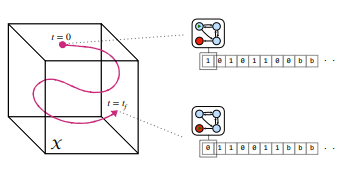
\includegraphics{System.png}
            \label{fig:my_label2}
        \end{figure}
    
\end{frame}

%Introduce AIT background
\begin{frame}{Algorithmic Information Theory}
\begin{block}{Kolmogorov Complexity}
The Kolmogorov complexity $K_U$ of a bitstring $x$ is the length of the shortest input program that when given to a UTM $U$ can produce $x$ as an output:
\begin{equation*}
    K_U(x) :=\min_{z:\phi_U(z) = x}\ell(z)
\end{equation*}
\begin{itemize}
    \item Measure of amount of information in $x$
\end{itemize}
\end{block}
\end{frame}

\begin{frame}{Algorithmic Information Theory}
    \begin{block}{Kolmogorov Complexity of Bitstring $x$}
    \begin{equation*}
        K_U(x) :=\min_{z:\phi_U(z) = x}\ell(z)
    \end{equation*}
    \end{block}
    \begin{block}{Kolmogorov Complexity of a Computable Function $f$}
    \begin{equation*}
        K_U(f) := \min_{M:\phi_M = f} \ell(\sigma_{U,M})
    \end{equation*}
    \end{block}
    \begin{block}{Conditional Kolmogorov Complexity of $x$ Given Bitstring $y$}
\begin{equation*}
    K_U(x|y) = \min_{z:\phi_U(z,y) = x} \ell(z)
\end{equation*}
\end{block}
\end{frame}

\begin{frame}{Algorithmic Information Theory}
    \begin{block}{Invariance Theorem}
    For distinct UTM $U$, $U'$:
        \begin{equation*}
            K_{U'}(x) = K_U(x) + O(1)
        \end{equation*}
        Thus, $U$ is usually omitted and we write $K(x)$ for Kolmogorov complexity of $x$
    \end{block}
\end{frame}

\begin{frame}{Algorithmic Information Theory}
\begin{block}{Incompressible string $x$}
If $x$ is incompressible, then 
\begin{equation*}
    K(x) = \ell(\text{print }x)
\end{equation*}
\begin{itemize}
    \item Any program capable of producing $x$ must contain $x$ explicitly
    \item $x$ is ``maximally dense" with information
\end{itemize}
\end{block}
 \begin{block}{Highly compressible string $\pi$}
    \begin{equation*}
        K(\pi) \le \ell \left( 6\sin^{-1}\left(\frac{1}{2}\right)\right) < \ell( \text{print }\pi)
    \end{equation*}
    \end{block}
\end{frame}

\begin{frame}{Algorithmic Information Theory}
\begin{block}{Input Distributions}
\begin{itemize}
    \item Input string $x$ as random variable with probability distribution $p_X$
    \item Important example: coin flipping distribution of TM $M$
    \begin{equation*}
        m_X^\text{coin}(x) := \begin{cases} 2^{-\ell(x)} &\text{if $x\;\in$ dom $\phi_M$}\\ 0 &\text{otherwise}\end{cases}
    \end{equation*}
    \item With normalizing constant $\Omega_M :=\sum_{x\in\text{ dom }\phi_M} 2^{-\ell(x)}$
    \begin{equation*}
        p_X^\text{coin}(x) = m_X^\text{coin}(x)/\Omega_M
    \end{equation*}
\end{itemize}
\end{block}
\end{frame}

\begin{frame}{Algorithmic Information Theory}
    \begin{block}{Shannon Entropy of Distribution $p_X$}
    \begin{equation*}
    S(p_X) = - \sum_{x\in X} p_X(x)\ln p_X(x)    
    \end{equation*}
    \begin{itemize}
        \item Measure of amount of information in $p_X$
        \item $\ln \frac{1}{p_X}$: "surprisal``, how unexpected, and hence informative, is $x$?
        \item $p_X(x)$: how often do we receive surprise $\ln p_X$
    \end{itemize}
    \end{block}
\end{frame}

\begin{frame}{Algorithmic Information Theory}
    \begin{block}{Entropy Production (EP)}
    The expected EP, written $\Sigma (p_X)$ of a physical process with initial state distribution $p_X$ and final state distribution $p_Y$ is:
    \begin{align*}
        \Sigma (p_X) &= S(p_Y) - S(p_X) + \langle Q \rangle_{p_X}/kT
    \end{align*}
    Thermodynamically reversible processes have $\Sigma (p_X)=0$. EP is always nonnegative.
    \end{block}
\end{frame}
%%%%%%%%%%%%%%%%%%%%%%%%5%References
\begin{frame}{References}
    \printbibliography
\end{frame}

 

\end{document}